We identified evolutionary singular strategies throughout parameter space for our parapatric model of speciation. The results of our analysis provided two major insights into the determinants of evolutionary branching. First, adaptive branching can be achieved through two modes; either driven by local adaptation to spatially heterogeneous fitness peaks, or by sympatric competition and frequency-dependent disruptive selection within patches. Which mode is at play highly depends on the combination of the trade-off between the utilization of the two resources and on the heterogeneity of the environment in resource availabilities. Second, assortative mating has a stabilizing effect on the evolutionary equilibrium and counteracts diversification.

\subsubsection*{Local adaptation versus competition-driven branching}

Figure \ref{fig:map_branching_points} shows the dynamics of the model throughout parameter space. The combination of ecological divergent selection, i.e. the strength of the trade-off between resources, and habitat symmetry, i.e. environmental heterogeneity, is important in determining whether branching can occur. In more homogeneous environments (high habitat symmetry), branching occurs within a certain range of trade-off strengths. As the landscape becomes more heterogeneous in what resources are available, weaker trade-offs favor branching. Not only the minimum level of selection needed to trigger branching decreases, leading to branching in the near-absence of selection in a highly heterogeneous landscape, but the level of selection at which the trade-off becomes too strong for branching to occur is also lower. This is because different modes of adaptive branching are favored in different habitat symmetry conditions.\\

Branching can occur in two different ways: (1) the population can diverge in ecological trait between the two habitat-patches, or (2) within each patch. Setting the dispersal rate $m$ to zero and analyzing the two patches separately allows to disentangle those two processes, at least in the absence of migration. Figure \ref{fig:map_divergence} shows that a higher asymmetry in resource availability between the two habitats favors different equilibrium trait values between the two patches, which leads to divergence across patches through local adaptation to different resources.\\

As habitat symmetry increases, however, branching becomes possible within each patch for a certain range of trade-off strengths (yellow layers in Fig. \ref{fig:map_divergence}) due to the disruptive effect of competition. If enough of the two resources are available within a patch, frequency-dependent selection favors the coexistence of two morphs, each specialized on one resource. For competition-driven branching to occur, the trade-off must be strong enough such that specialist strategies (either $-1$ or $+1$) are advantaged over generalist strategies ($x = 0$). In a completely homogeneous environment, this transition happens exactly at a divergent selection coefficient value of $s = 0.5$, which is the lower bound observed in Fig. \ref{fig:map_branching_points} and \ref{fig:map_divergence}.\\

A stronger trade-off does not always favor branching, however. If the trade-off is above a certain threshold, selection becomes too strong for any kind of branching to occur (be it through local adaptation or competition). Figure \ref{fig:pairwise_invasibility_s} illustrates why this is. The branching point is the generalist strategy $x = 0$, meaning that a monomorphic population will first converge to this trait value before becoming polymorphic. As the trade-off increases in strength, either specialist strategies $-1$ and $+1$ become stable alternatives that are more advantageous than a generalist strategy for populations starting with nearby those specialist strategies. Meanwhile, the branching point will only be able to attract populations that are more and more restricted to the direct neighborhood of the generalist strategy. This explains why branching does not always happen for a population starting off as a $-1$ specialist, even if a branching point still exists at $x = 0$, in Figures \ref{fig:map_branching_points} and \ref{fig:map_divergence}. Above a certain threshold in trade-off strength, the branching point loses its convergence stability and becomes an evolutionary repeller, i.e. populations get trapped at specialist strategies (which one depends on the starting conditions) because the evolution of a generalist type, which is needed to undergo branching, is selected against.\\

Migration between the two patches generally brings the behavior of the model closer to that of a scenario with a homogeneous landscape (Fig. \ref{fig:map_branching_points}). Therefore, it quite possibly expands the range of conditions under which branching through competition can occur, but this remains to be tested.

\subsubsection*{Assortative mating prevents diversification}

Although assortative mating is a necessary ingredient to allow reproductive isolation in sexual organisms in the presence of gene flow, this effect strongly depends on the genetic variation in the population. Assortative mating with respect to ecotype typically reinforces branching and subsequent divergence, provided that there is enough variation in trait values in the population so that mutant individuals do not suffer too much the cost of being rare. Genetic variation is often very low in adaptive dynamics models, where the resident population is monomorphic with respect to the evolving trait. As such, assortative mating inevitably selects against mutants that deviate in trait value from the resident, because male residents are optimally suited to female preferences (their phenotypes are in complete match). This is what we showed in Equation ..., and it is also illustrated in Figures \ref{fig:map_branching_points}, \ref{fig:map_divergence}, and \ref{fig:pairwise_invasibility_alpha}, where increasing the sexual selection coefficient, i.e. the degree of assortative mating, can increase the stability of the branching point, eventually turning it into an evolutionarily stable strategy.

\begin{figure}
    \centering
    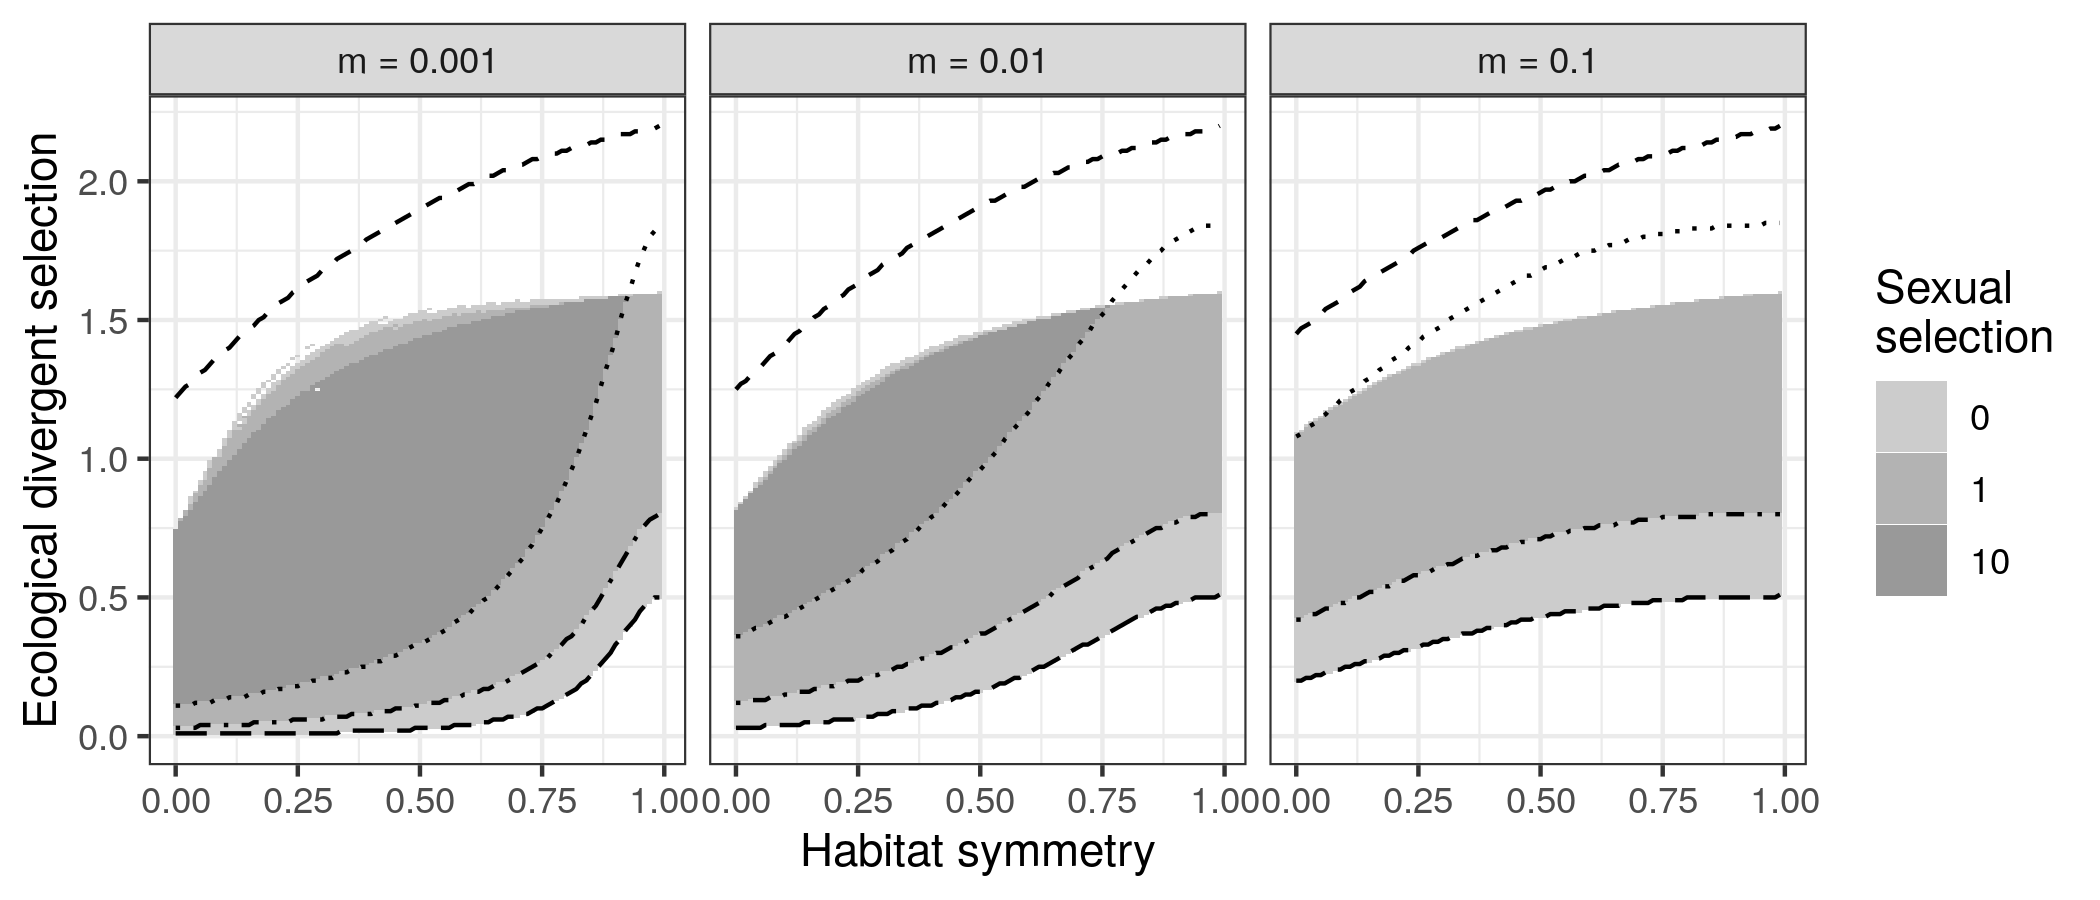
\includegraphics[width=\textwidth]{figures/map_branching_points}
    \caption{Branching throughout parameter space for three values of the dispersal rate $m$. Sexual selection increases the stability of evolutionary equilibria and therefore turns branching points into stable strategies. Shades of grey indicate the highest tested level $\alpha$ of sexual selection at which branching still occurs when a population is initially a specialist of the first resource ($x = -1$). Dashed lines expand the borders of the grey areas to show the full extent of where branching can theoretically occur, i.e. whether any branching point exists, irrespective of the starting trait value. Parameters, $a = 400$, $b = 100$, $d = 0.2$, $\alpha = 0$.}
    \label{fig:map_branching_points}
\end{figure}

\begin{figure}
    \centering
    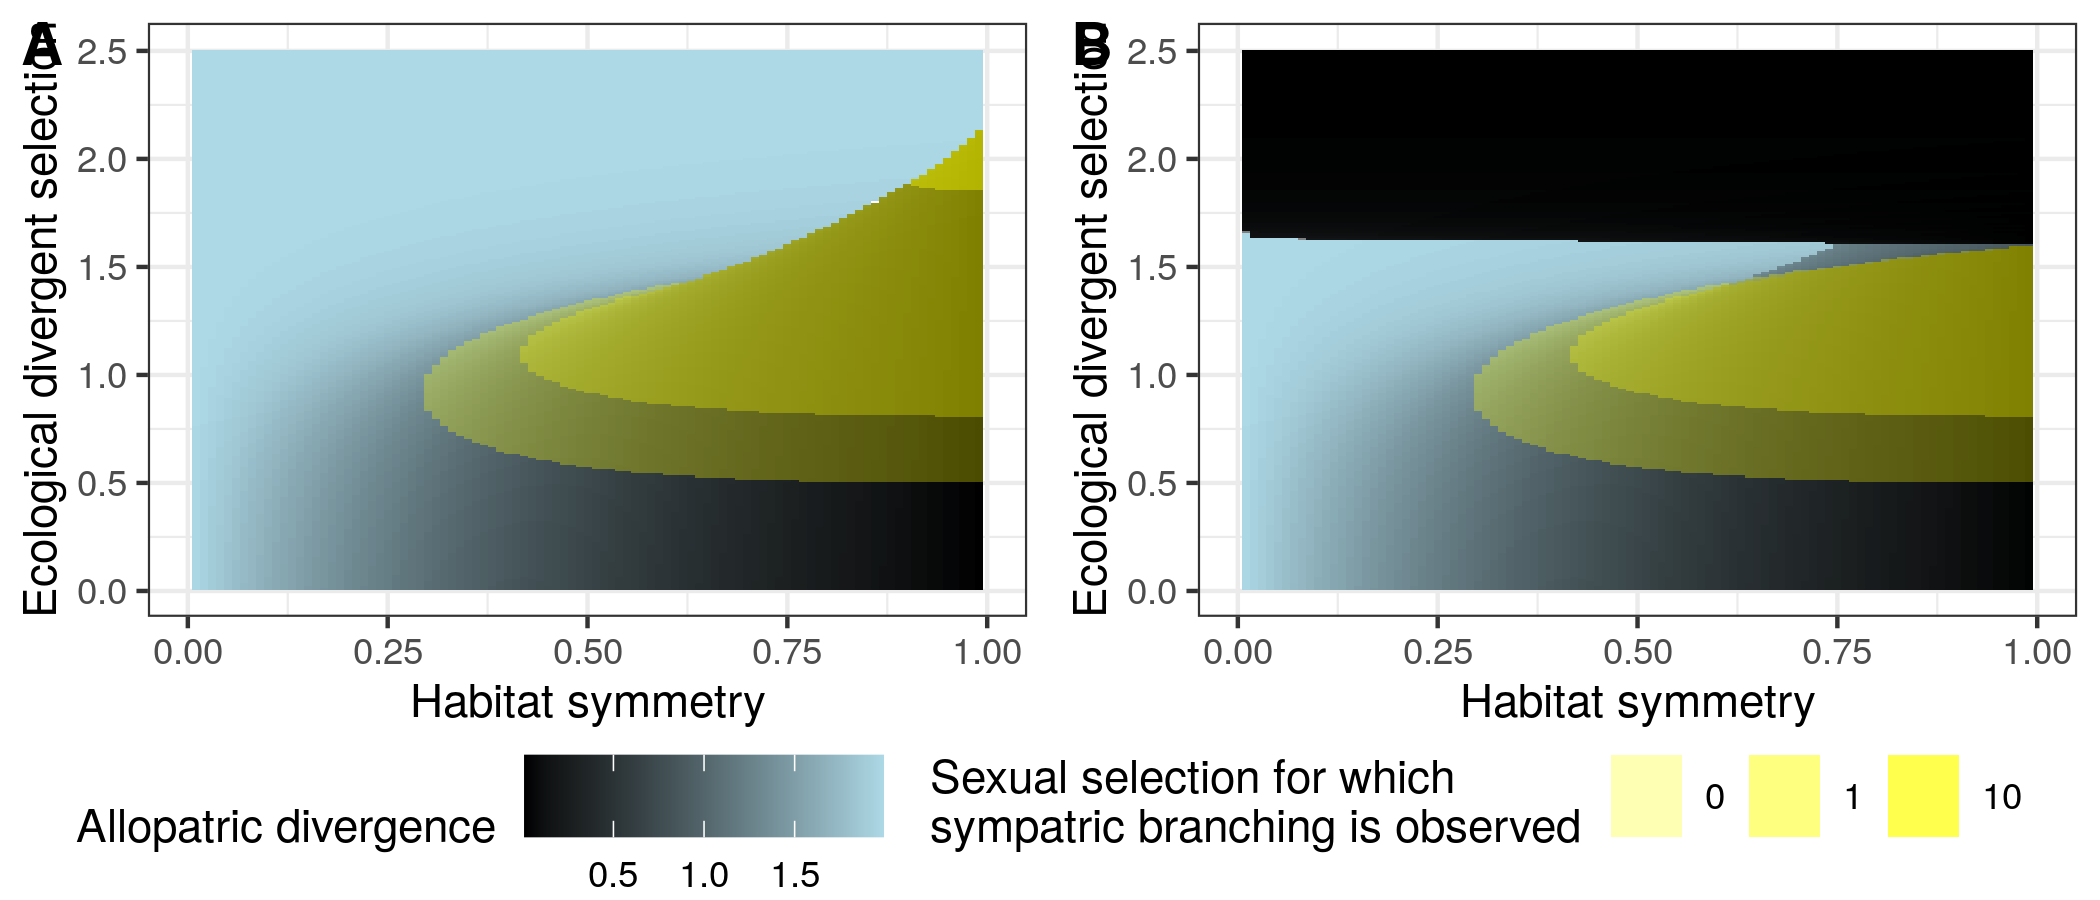
\includegraphics[width=\textwidth]{figures/divergence_across_patches}
    \caption{The divergence in ecological trait between the two patches in the absence of dispersal is shown across parameter space, when the two habitat-populations are initialized with trait value (A) $x = 0$ or (B) $x = -1$. Allopatric divergence is measured as the difference in attained equilibrium between the two habitats. Transparent yellow layers show regions of parameter space where both populations undergo within-patch branching due to competition after reaching their convergence-stable equilibrium. Increasing assortative mating reduces the parameter space where competition-driven, within-patch branching is possible.}
    \label{fig:map_divergence}
\end{figure}

\begin{figure}
    \centering
    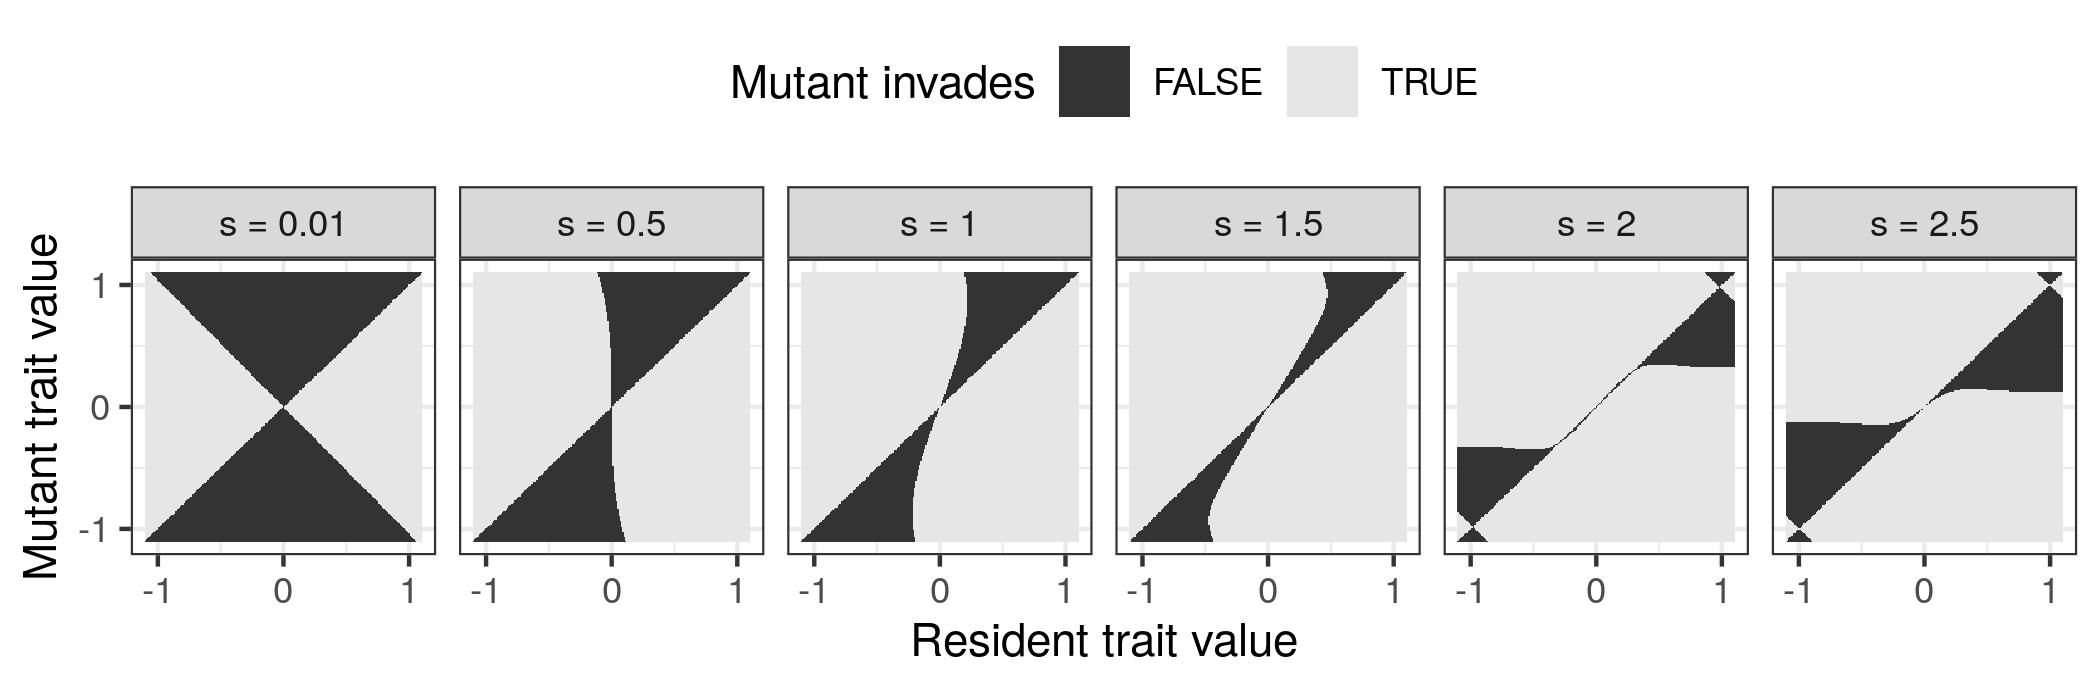
\includegraphics[width=\textwidth]{figures/pairwise_invasibility_plots_test_s}
    \caption{Pairwise invasibility plots showing the effect of the ecological divergent selection $s$ on the singular strategies. The strategy $x = 0$ is a branching point only for intermediate values of $s$. If $s < 0.5$, the population converges to the stable generalist trategy $x = 0$. As $s$ continues to increase, the specialist strategies $-1$ and $+1$ become stable alternatives to branching (panel $s = 2$). At some point, the strategy $x = 0$ becomes a repellor and the only the specialist strategies remain convergence-stable. Parameter values, $a = 400$, $b = 100$, $h = 1$, $d = 0.2$, $m = 0.01$, $\alpha = 0$.}
    \label{fig:pairwise_invasibility_s}
\end{figure}

\begin{figure}
    \centering
    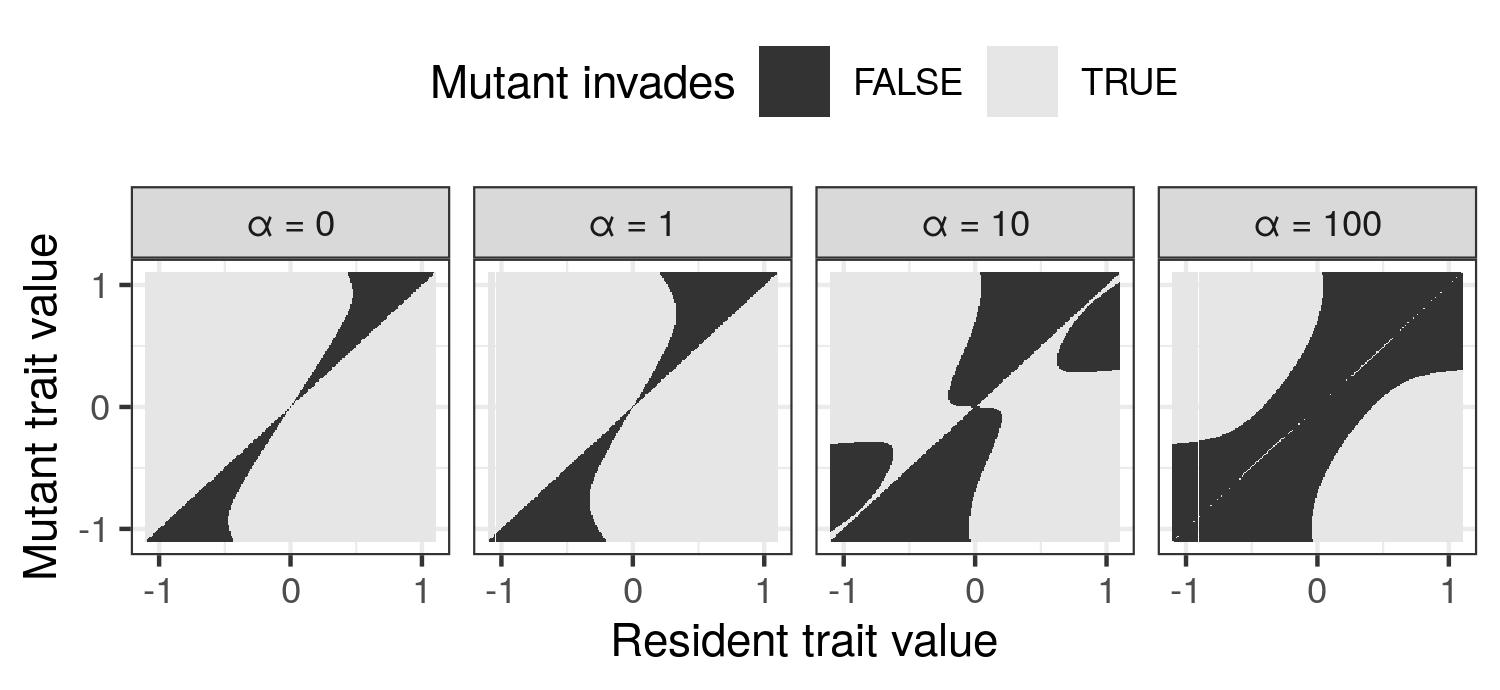
\includegraphics[width=\textwidth]{figures/pairwise_invasibility_plots_test_alpha}
    \caption{Pairwise invasibility plots showing the stabilizing effect of assortative mating. Increasing the sexual selection coefficient $\alpha$ turns the branching point at $x = 0$ into a stable strategy, somewhere between $\alpha = 1$ and $\alpha = 10$. Parameter values, $a = 400$, $b = 100$, $h = 1$, $s = 1.5$, $d = 0.2$, $m = 0.01$}
    \label{fig:pairwise_invasibility_alpha}
\end{figure}